%=====================================================
\begin{frame}{3.1.1. Декларируемый уровень доверия к руководству (сводный результат) }

\tiny

На диаграмме представлен сводный результат по вопросу Б18:
\bigskip


Б18. Согласие с тем, что руководство образовательной организации защищает интересы респоднента и заботится о нем: ``Согласны ли Вы с тем, что руководство образовательной организации защищает Ваши интересы и заботится о Вас?''
\bigskip

\begin{columns}
\begin{column}{0.4\textwidth} 
\centering
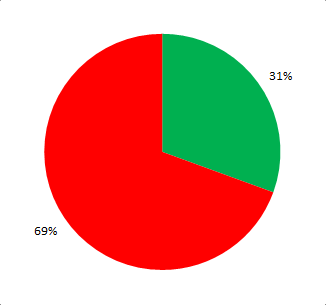
\includegraphics[width=4cm, height=4cm]{diag.png}
\end{column}
\begin{column}{0.6\textwidth} \begin{tabular}{l} 
 Ответили утвердительно   \\ 
(``да'' или ``скорее да, чем нет'')  ---   \valCAAyesNum\ (\valCAAyesNumP\%) \\ [0.3cm]
 Ответили отрицательно  \\ 
 (``нет'' или ``скорее нет, чем да'') ---  \valCAAnoNum\ (\valCAAnoNumP\%) \\ 
\end{tabular}
\end{column}
\end{columns}

\end{frame}


